\documentclass[a4paper,10pt]{article}
\usepackage{ctex}
\usepackage{fancyhdr}
\usepackage{mflogo,texnames}
\usepackage[latin1]{inputenc}
\usepackage{graphicx}
\usepackage{amssymb}
\usepackage{epstopdf}
\usepackage{listings}
% 插入伪代码
\usepackage[linesnumbered,boxed]{algorithm2e}\usepackage{color}
\definecolor{keywordcolor}{rgb}{0.8,0.1,0.5}
\definecolor{webgreen}{rgb}{0,.5,0}
\usepackage{geometry}
\geometry{left=3.18cm,right=3.18cm,
    top=2.54cm,bottom=2.54cm,
    head=1.5cm,foot=1.75cm}
\usepackage{multirow}
\pagestyle{fancy}
\lhead{学号:1401214342}
\chead{姓名: 韩喆}
\rhead{}
\lfoot{Han Zhe(icst@pku)}
\cfoot{iampkuhz@gmail.com}
\rfoot{\thepage}

% word page layout
%\usepackage[top=2.54cm, bottom=2.54cm, left=3.18cm, right=3.18cm]{geometry}
\title{My First \LaTeX{} article}
\begin{document}
\begin{center}
\LARGE 算法课第 3次作业
~\\
\end{center}

\begin{center}
 \begin{tabular}{|c|c|c|c|c|c|c|}
\hline
      & 题目1 & 题目2 & 题目3 & 题目4 & 题目5 & 总分\\ \hline
 \multirow{2}{*}{分数} &\multirow{2}{*}{} &\multirow{2}{*}{} &\multirow{2}{*}{} &\multirow{2}{*}{} &\multirow{2}{*}{} &\multirow{2}{*}{}\\
 & & & & & & \\ \hline
 \multirow{2}{*}{阅卷人} &\multirow{2}{*}{} &\multirow{2}{*}{} &\multirow{2}{*}{} &\multirow{2}{*}{} &\multirow{2}{*}{} &\multirow{2}{*}{}\\
 & & & & & &  \\ \hline
\end{tabular}
\end{center}
\vspace{20pt}
\section{诈骗检测}
  \normalsize
  \subsection{$O(n\log n)$算法}

  \paragraph{算法及正确性说明}算法思想: 递归查找每一半中出现次数最多的元素, 出现次数超过一半的元素, 肯定在任意二分中, 在其中某一半中是出现次数最多的元素(否则, 出现次数最多的元素在两半中都不超过一半, 在总体中出现次数也不超过一半, 矛盾). 我们二分查找出现次数最多的元素,然后进行最终判断, 将其与其他所有元素比较判断其出现次数.\\
  1. 将所有元素平分成2组(总数为奇数则一组比另一组多一个元素). 对于每组,递归返回每组内出现次数最多的两个元素$a_1, a_2$. 然后将$a_1, a_2$和2个组的所有元素比较, 算出$a_1, a_2$出现次数, 取两者中出现次数多的返回. \\
  2. 判断1.中求得的元素是否出现超过$n/2$次: 根据第一步得到集合中出现次数最多的元素$a_0$, 将其和集合中的所有元素比较. 如果其出现次数大于$n/2$, 则答案为存在; 否则, 不存在.
  \paragraph{复杂度分析}对于元素大小为m的集合$R(m)$, 假设其复杂度为$T(m)$. 开始是元素个数为n, 处理复杂度$T(n)$, 递归的复杂度为$2\times T(n/2)$, 找到两个元素后和其他元素比较,需要$2\times n$. 递推式为 
  $$T(n)=2\times T(n) + 2n$$
  又有$T(1) = 0$从而得到$T(n)=2n\times\log n$, 比较次数复杂度为$O(n\log n)$. \\
  在每个阶段, 只需要2个空间存储每组的最频繁元素和2个空间存储他们的出现次数,阶段结束后不需要额外的空间.所以空间复杂度为
  $$O(2+4+8+...+2^k)=O(2n)=O(n)$$
  其中$2^{k-1}<n$
  
  
  \subsection{$O(n)$算法}
  \begin{figure}[h]
  \centering
  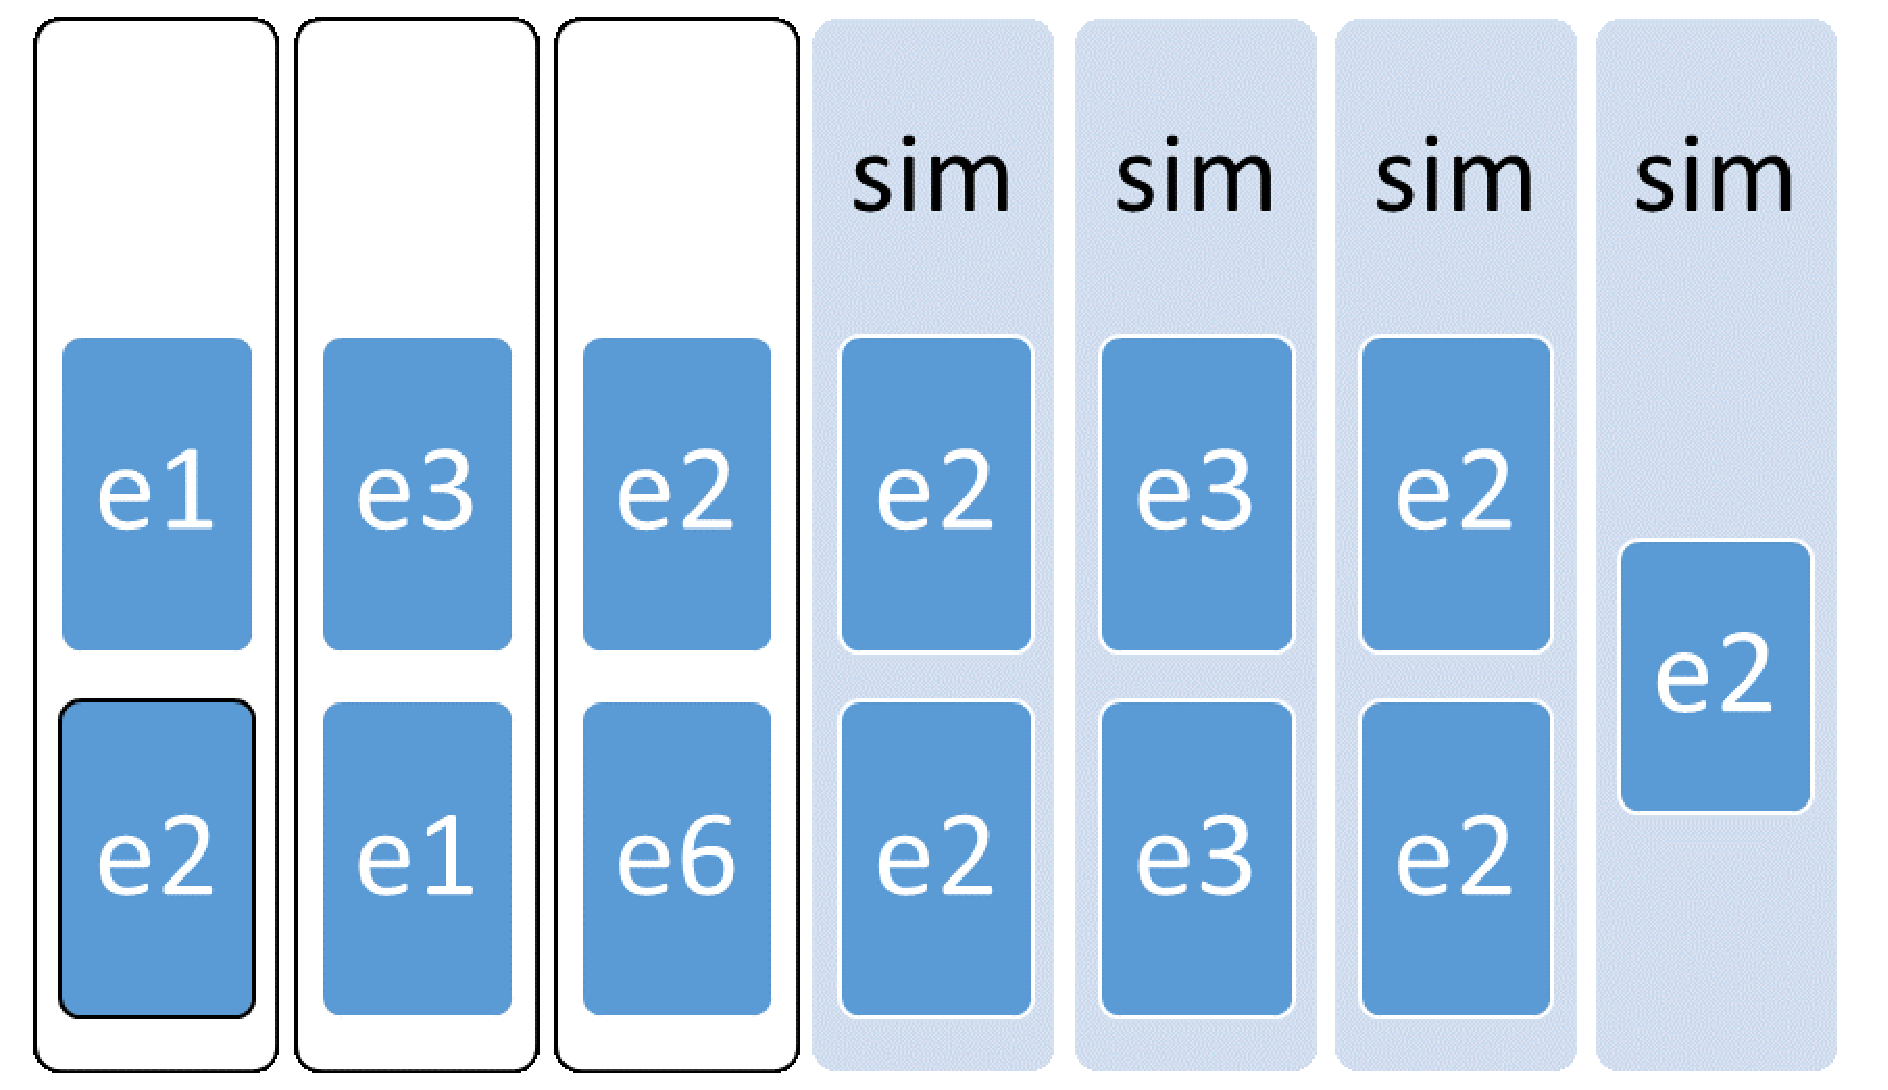
\includegraphics[width=0.8\textwidth]{hw3_p1}
  \end{figure}
  \paragraph{算法及正确性说明}
  算法思想: 假如存在超过n/2次的元素, 则将所有元素配对后, 一定存在某些配对, 对中的2个元素相同, 且出现次数最多的元素一定在相同配对中出现(因为出现次数超过一半), 并且在相同配对中任然满足出现次数过半的性质(下面会证明). 我们先找到这个可能的元素, 然后再算他的出现次数是否满足超过一半要求.\\
  1. 递归查找该元素: 将所有元素两两配对. \textbf{如果剩下一个元素, 将其与其他所有元素比较一遍, 如果是出现超过一半的元素, 返回, 否则删除}. 假如没有一对元素相同, 说明不存在出现次数超过一半的元素(显然); 假如存在, 则可能的出现次数超过n/2的元素一定在重复元素对中出现(剩下的元素每对至多只有一个是出现次数最多的元素,总次数小于n/2). 并且, 在重复的''对''中, 其出现次数占''对''数的一半以上(因为在没有配对成功的对中该元素至多出现一半, 要想在总的元素中出现次数超过一半, 只可能在重复对中出现超过一半).\\
  2. 在上面得到的重复对中, 每对只取一个元素, 递归查找该元素\\
  3. 判断上面查找得到的元素的出现次数, 和所有其他元素比较一次. 如果其出现次数大于$n/2$, 则答案为存在; 否则, 不存在.
  \paragraph{复杂度分析}
  假设有k对相同, 需要判断$\frac{n}{2}$次, 有 
  $$T(n)=T(k)+\frac{3n}{2}\leq T(n/2)+\frac{3n}{2}$$
  所以得到$$T(n)=3n\times (1+\frac{1}{2}+...+(\frac{1}{2})^{\log n})=3n\times(2-(\frac{1}{2})^{\log n})<6n$$
  所以比较次数复杂度为$O(n)$\\
  而递推的时候需要一半的空间递推得到候选元素, 所以空间复杂度(和上面类似的等比数列,证明类似)为$O(n)$
  
  
\section{重要的逆序}
  \paragraph{算法即正确性说明} 算法思想: 改进归并排序求逆序对时合并的过程, 合并时做两次, 第一次算重要逆序对数(不是真的合并), 最后一次才是真正的合并.
  \begin{center}
   总的逆序对数=2组的组内重要逆序对数$+$组间重要逆序对数
  \end{center}
  1. 分: 将元素分成两组, 每组递归求组内的重要逆序对数, 并将每组元素排好序.\\
  2. 和: 两组排好序的元素分别为$\mathbb{R}_1, \mathbb{R}_2$, 先将$\mathbb{R}_2$的元素大小全部乘以2,和$\mathbb{R}_1$按照算逆序对的归并方式计算组间逆序对数(两组元素各自有一个指针从左往右比较元素大小, 每次两个指针中指向较小值者的指针向右移动一位直到某一个指针到达末尾; 如果后一个数组的指针指向的数值较小, 则其比前一个数组指针指向的位置及其之后的元素都小, 逆序对数需要加上前一个数组的当前剩余元素个数), 得到的就是组间重要逆序对数. 然后再将$\mathbb{R}_2$的元素变成原来的大小重新做一次(不过不仅仅比较大小, 还要做归并排序), 此时得到排好序的数组.
  \paragraph{复杂度分析}
  对于元素大小为m的集合$R(m)$, 假设其复杂度为$T(m)$. 开始是元素个数为n, 处理复杂度$T(n)$, 递归的复杂度为$2\times T(n/2)$, 合并是进行2次,每次比较n次,需要$2\times n$. 递推式为 
  $$T(n)=2\times T(n/2) + 2n$$
  又有$T(1) = 0$从而得到$T(n)=2n\times\log n$, 比较次数复杂度为$O(n\log n)$. \\
  合并阶段, 第一次计算重要逆序对数时不输出结果, 不需要额外的数据存放排序结果, 计算完后只需要将$\mathbb{R_2}$的元素在原来位置上除以二即可. 第二次合并时需要n个空间存储合并后的数组.所以空间复杂度为
  $$O(n(1+\frac{1}{2} +...+(\frac{1}{2})^{\log n})=O(2n)=O(n)$$\\
  
\section{数据库的中位数}
  \paragraph{算法及正确性说明} 算法思想: 二分查找中位数. 设两个数组为A, B, 数组A的第k大个元素值为A[k]\\
  1. 开始时令$k=\lceil\frac{n}{2}\rceil$, 区间长度L=n, (1)A[k]<B[k]. 对于A[k], 在数组A中有n-k个元素排在他的后面, 在数组B中, B[k]及其之后的数都大于它. 所以数据库中至少有$n-k+(n-k+1)=2n+1-2k=2n+1-2\lceil\frac{n}{2}\rceil\geq n$, 所以数组A中在A[k]之前的元素至少有$n+1$个元素比他们大, 所以中位数不可能在数组A的前k-1个元素中. 同理, 中位数不可能在数组B的后n-k个元素中,所以中位数的搜索范围变为$A[k, k+\lceil\frac{n}{2}\rceil-1]$和$B[k-\lceil\frac{n}{2}\rceil+1, k]$(2)A[k]$\geq$B[k], 同上, 只需要考虑两个数组各自的另一半区间.\\
  2. 递归查找中位数直到区间长度变为1. 此时中位数就是A[k],B[k]中的较小者.\\
  伪代码表示为: Algorithm1
  \begin{algorithm}
  \caption{medianFind}
   medianFind($n$, $a$, $b$)\\
  \Begin{
    $k=\lceil\frac{n}{2}\rceil$\;
    \lIf {$n$=1} {then \Return $min(A[k], B[k])$}
    \lIf{A[k]<B[k]}
      {\Return medianFind($k$, $a+\lfloor\frac{n}{2}\rfloor$, $b$)}
    \lElse{ \Return medianFind($k$, $a$, $b+\lfloor\frac{n}{2}\rfloor$)}
    }
    \end{algorithm}

  \paragraph{复杂度分析}
  循环的次数最多为$\log n$次, 每次查询2次数据库, 所以时间复杂度为$O(\log n)$. 因为每个递归函数内的空间复杂度为O(1), 递归$\log n$次, 所以空间复杂度也为$O(\log n)$\\
  
  
\section{局部最小点}

  \begin{figure}[h]
  \centering
  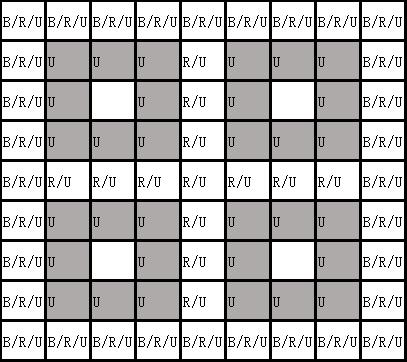
\includegraphics[width=0.8\textwidth]{hw3_p4}
  \end{figure}
  \paragraph{算法及正确性说明} 算法思想: 将网格以''田''字型边框(中间一行,中间一列和最外面一圈)为边切分,分成5个部分:边框部分(R)以及被边框切分出的4个方图部分(S). 如果边框上存在局部最优点, 则算法停止(下面证明); 否则, 证明4个部分中有一个部分存在局部最优点, 对其及其边框递归查找.
  \subparagraph{最优性MinG}邻接图G(边长大于等于3)满足性质MinG, 如果: 最外面一圈的点集(B)相邻点点集A上存在在一个点v, v上的值小于所有B上点的值.
  \subparagraph{满足MinG的邻接图中查找局部最优点的复杂度}邻接图G满足MinG. 按MinG的定义将G分为5个部分.查找[方图(S)边框以及框图(R)](合称为U)中值最小的节点v. 则:\\ 
  (1)v在框图R上, 则v一定在中间一行或中间一列(U中包含B的所有邻接点,按照MinG性质存在点值小于B上的所有点, 又其在R上,所以其只可能在中间行或中间列中), 由U的集合构成知, v的上下左右点如果存在, 必然都在U内, 所有v是局部最优点, 找到 \\
  (2) v在方图S的边框上. 则取该方图(抛弃其余3个方图), 连同R中在该方图周围的点组合成为一个满足MinG的边长为$\lfloor\frac{n}{2}\rfloor+1$,递归可以求得节点v *\\
  \textbf{*算法一定会停止(找到). 因为: 边长大于等于4时, 就可以找到小方图(等于4时只有1个小图, 其余都是4个. 又因为小方图(边长至少为1)连同R上在该方图周围的点(使边长增加2)构成的正方形边长至少为3, 所以最终递归结束时的边长一定为3(也有可能不存在小方图, 也就是说v点在S的边框上, 就是情况(1)). 而当边长为3时中心点的四周就是边界, 中心点就是局部最优点, 结束} 
  \subparagraph{复杂度分析} 每个递归过程,假设方图边长为n, U的元素个数为$O(n)$, 找到其中最小点的时间复杂度为$O(n)$, 递归子图的边长为$\lfloor\frac{n}{2}\rfloor+1$, 所以有 
  $$T(n)=T(\lfloor\frac{n}{2}\rfloor+1)+O(n)$$
  所以$T(n)=O(n)$.
  \subparagraph{简要证明$T(n)$}
  对于n较大时$T(\lfloor\frac{n}{2}\rfloor+1) < T(\frac{3}{4}n)$, 所以
  $$T(n)<T(\frac{3}{4}n)+O(n)<...<O(n)\times(1+ \frac{3}{4} + (\frac{3}{4})^2+...)<4O(n)=O(n)$$\\
  
   
\section{矩阵乘法}
  \paragraph{(1)} 根据题目思路, 转换为大小为$\frac{n}{3}$的子问题后, 子问题的一次乘法实际上变成了一个3*3的矩阵乘法, 子问题的一个乘法代价为k, 所以递推式为
  $$T(n)=k\times T(\frac{n}{3})$$
  且$T(3)=k$, 令$n= 3^m$,则有 
  $$T(n)=k\times T(\frac{n}{3})=k\times k\times T(\frac{n}{9})=...=k^{m-1}T(3)=k^m=k^{\log_3 n}$$
  令$k=3^l$, 则$(3^l)^{\log_3 n}=3^{l\log_3 n}=(3^{\log_3 n})^l=n^l=n^{\log_3 k}$, 时间复杂度为$O(n^{\log_3 k})$
  \paragraph{(2)} 由(1), 令$n^{\log_3 k}\leq n^{\log 7}$得:
  $$ \Rightarrow \log_3 k \leq \log 7 $$ 
  $$\Rightarrow k \leq 3^{\log 7} \approx 21.85$$
  所以k最大为21
\end{document}
